% Chapter 3

\chapter{From Sequence to Metabolic Reconstruction} % Main chapter title

\label{Chapter3} % For referencing the chapter elsewhere, use \ref{Chapter3}

%---------------------------------------------------------------------------------------- This is the pipeline
%---- Overview of algorithm process ---
\indent\indent ASGARD and MetModel are tools that perform genome annotation, and metabolic pathway reconstruction respectively. Both tools do their job well but it is not easy or intuitive to use them and especially not together.  For starters, neither of these tools provide adequate documentation on how to use them or the specific file formats and data that they require to run.  Next, they don't integrate well on their own so it was not possible to start from the raw nucleotide sequence data and build a metabolic model from there before our work. Now while the process is still not completely automated, that decision was actually intentional as it is helpful to be able to review the output from each step in the workflow in order to ensure nothing is missing and manually add or remove reactions or metabolites if need be.  Figure 3-1 shows an overview of the pipeline and the steps that MetModel uses to perform FBA and generate the KGML reaction maps.  Our specific contributions are highlighted in yellow, and the scoring function which was developed by Stephen Wunsch and then incorporated into the pipeline is highlighted in green\citep{wunsch_stephen_a._scoring_2016}.\\
% * <jpbrooks@vcu.edu> 2016-08-31T02:35:17.916Z:
%
% > respective jobs
%
% describe the jobs
% ADD Wunsch citation here
% ^ <norrissw@vcu.edu> 2016-09-01T02:47:10.477Z.
\begin{figure}[h]
\centering
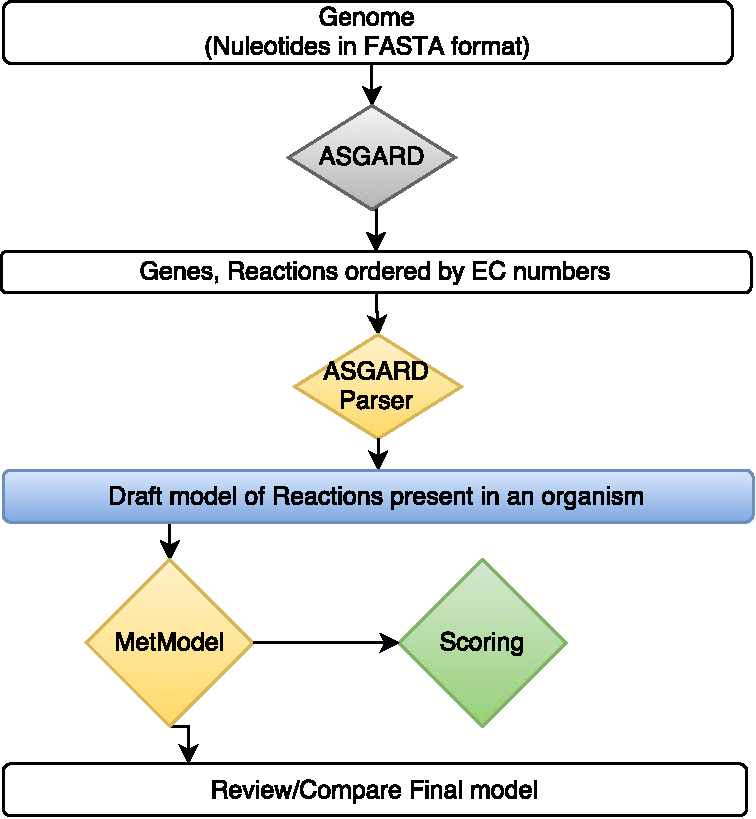
\includegraphics{Figures/Pipeline}
\decoRule
\caption[Pipeline Workflow]{This shows the workflow used to reconstruct a metabolic network starting from just the nucleotide sequence of an organism's genome. My specific contributions are highlighted in yellow, and the collaborative effort on the scoring mechanism is highlighted in Green.}
\label{fig:Pipeline}
\end{figure}

%---- The two main contributions are: ---
\section{ASGARD Parser}

\indent As mentioned before, ASGARD is a tool for determining open reading frames and then annotating genes, then uses this protein product information to determine the reactions present in the gene.  It works by supplying a FASTA formatted file, and the output is a BED file which contains the enzyme commission numbers (EC) that were predicted to be present in the organism.  This is a big step toward building a complete pathway model, but there were still missing steps before a model could be generated.  First, a python script was developed and used to parse the EC numbers from the output, and searched within the new reference database for the associated reactions, pathways, and if possible genes/gene products associated with them.  This information was then used to build the list of reactions needed to run MetModel.\\

%----- 1. Call ASGARD, get EC Numbers, Build 'Model' for MetModel, Call MetModel Pipeline through met_model script------
%-------- A Table showing pathway/reaction counts would be good here %----------
\section{MetModel Pipeline}

\indent\indent Once the data from ASGARD was formatted properly it could now be used with the MetModel pipeline.  In order to use MetModel originally you either had to create your own scripts and call the appropriate functions or for convenience four separate static scripts were written as example usages and each had to be tailored specifically to the model that was being run and each script performed a single step which needed to be executed independently and in order. As a part of this work all of the function calls, data, and information that was contained in these four separate scripts were incorporated into one Python script which created an user friendly, reusable software tool. The new script uses command line arguments to run different procedures and can be run dynamically without having to alter the code of the scripts themselves.  Doing this created a semi-automated process in which a user can use to pause at each step if he or she wishes to manually intervene or review the files produced before completing the entirety of the MetModel FBA process. \\ 
% * <jpbrooks@vcu.edu> 2016-08-31T02:37:16.572Z:
%
% > MetModel was originally used in four separate static scripts that all had to be run independently.
%
% No, MetModel is a collection of Python functions.  There were four convenience scripts created to call these functions.
%
% ^ <norrissw@vcu.edu> 2016-09-01T02:49:08.418Z.
\indent This tool we created allows the user to also select which steps in the pathway to perform, the default being all four.  Step 1 the MetModel pipeline adds transport reactions and if desired you can even attempt to build a model from this information. In step 2 we perform gap filling to complete the pathways and use FBA to determine the reaction rates and fluxes. In step 3, if experimental data is available it can be incorporated. In Step 4, the KGML maps are rendered.	These models were then scored and validated using the scoring function implemented by Stephen Wunsch\citep{wunsch_stephen_a._scoring_2016}.  \\
% * <jpbrooks@vcu.edu> 2016-08-31T02:39:24.708Z:
% again add WUNSCH citation
% > the final FBA is performed
%
% It's the same FBA instance, so really Step 4 is only to generate KGML maps.
%
% ^ <norrissw@vcu.edu> 2016-09-01T02:50:04.172Z.
% * <jpbrooks@vcu.edu> 2016-08-31T02:38:46.862Z:
%
% > FBA to generate a model.
%
% FBA does not generate a model.  It provides reaction rates/fluxes.
%
% ^ <norrissw@vcu.edu> 2016-09-01T02:50:05.159Z.

\indent The scoring method is designed to give a relative confidence score in the pathways that were included in the final model. It is the result of a collaborative effor between Dr. Stephen Fong, Stephen Wunsch and myself and was ultimately implemented by Stephen Wunsch, a PSM Bioinformatics graduate student\citep{wunsch_stephen_a._scoring_2016}
% ---It is the result of a collaboratative effort between Dr. Stephen Fong, myself and Stephen Wunsch. -- I don't know how to say this?
The method he developed works by using BeautifulSoup, a Python library and framework for webscraping, similar to Scrapy. It takes an individual reaction within a network and uses BeautifulSoup to seek out publications that provide experimental evidence of that reaction within the pathway and organism.  The more unique data it can discover the higher the score.  It then outputs these scores on a scale of 1-10, 1 being the lowest and 10 being the highest. A score of 10 indicates that the gene, protein, and reaction all have at least one primary journal article supporting them that contains experimental evidence that explicitly shows that the gene products and reactions are present in the organism. The score decreases from there when evidence cannot be found for example, a score of 5 indicates that the gene-protein reaction (GPR) have been associated with multiple EC numbers but are without publications that provide direct experimental evidence to support them.\\